\section{The Data Risk Exposure}
\label{sec:value}

\subsection{From Coefficients to Market Value}

The baseline coefficient can be translated into an implied change in firm value. By the definition of Tobin's Q, $Q_{it}=(M_{it}+D_{it})/A_{it}$, where $M$ is equity market value and $D$ is total liabilities. For small changes, the proportional change in log Tobin's Q is approximately the proportional change in the sum of equity value and liabilities. For a high-TDDI firm $i$, using 2021Q1 as the base period, the implied market-value loss is
\begin{equation}
\widehat{\Delta M}_i=\hat{\beta}\left(M_{i,2021Q1}+D_{i,2021Q1}\right),
\label{eq:dmv}
\end{equation}
where $\hat{\beta}=-0.0917$ is the binary coefficient in column (1) of Table \ref{tab:main}. Summing $\widehat{\Delta M}_i$ over the 100 high-TDDI firms gives the sample-level data risk exposure. The confidence interval uses the standard error of $\hat{\beta}$ times $\pm1.96$ and the same base-period value.

Table \ref{tab:value} reports the results by industry. The total implied market-value loss for high-TDDI firms is about RMB 203.7 billion, with a 95\% confidence interval of RMB 54.7--352.8 billion. Software development has the largest loss (RMB 61.5 billion), followed by communication services (RMB 35.2 billion), advertising and marketing (RMB 25.7 billion), IT services (RMB 23.1 billion), and gaming (RMB 16.0 billion). The ranking differs from the TDDI ranking because absolute losses depend on both exposure intensity and market value. Advertising has the highest average TDDI, but its high-TDDI firms are smaller on average, so the absolute loss is lower than in software and communication services.

\begin{figure}[htbp]
\centering
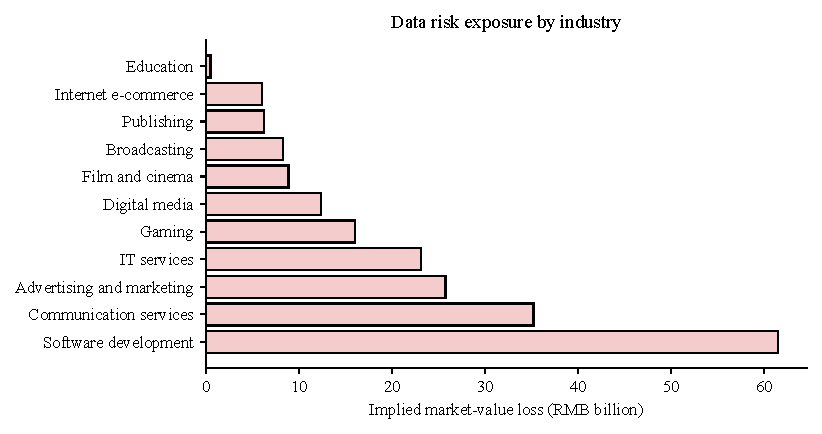
\includegraphics[width=0.9\textwidth]{fig5_value_by_industry.pdf}
\caption{Implied market-value loss of high-TDDI firms by industry. Bars are the implied loss from applying the baseline log Tobin's Q coefficient ($-0.0917$) to the sum of 2021Q1 equity market value and liabilities. Units are RMB billion. The sample contains the 100 high-TDDI firms.}
\label{fig:value}
\end{figure}

\subsection{Interpreting the Estimate}

The RMB 203.7 billion figure is a data risk exposure, not the total value of data assets. It has three interpretations. First, it is a firm-side private cost: the privacy regime reduces the expected rents from third-party data, and the market adjusts valuations accordingly. It does not include the consumer privacy benefits or the welfare effects of the regulation. Second, it covers a narrow asset class: third-party tracking, advertising, and data-service data. First-party data, algorithms, brands, network effects, and user relationships are outside the calculation. Third, it is a market revaluation of future rents, not the historical cost of acquiring data or the replacement cost of data infrastructure.

For data-asset accounting, the estimate provides an operational benchmark. Current data-asset recognition focuses on internally generated data resources and uses cost or income approaches. The risk exposure from third-party data dependence is not yet a standard accounting item. Our results show that third-party data dependence is a measurable, priceable, and industry-specific risk factor. For regulators, the magnitude indicates that the cost of privacy regulation is not borne only by consumers; B2B data-service firms and data-dependent software and communication firms bear a substantial adjustment cost. For investors, the TDDI can serve as an ex ante observable risk indicator for data-intensive firms.

The estimate can also be read as a lower bound on the value of the affected data. It captures only the portion of data rents that the market expected to be lost under the 2021 regime. If firms adapt by building first-party data, using privacy-enhancing technologies, or changing their advertising mix, the long-run loss may be smaller. If the shock also reduced the option value of future data-driven products, the total value of the affected data would be larger. The point estimate is a benchmark, and the confidence interval reflects the uncertainty in the valuation coefficient.

\begin{table}[htbp]
\centering
\small
\small
\setlength{\tabcolsep}{3pt}
\caption{Implied market-value loss of high-TDDI firms by industry.}
\label{tab:value}
\begin{threeparttable}
\begin{tabular}{lccccc}
\toprule
Industry & Firms & Market value (RMB bn) & Implied loss (RMB bn) & 95\% lower & 95\% upper \\
\midrule
Software development & 20 & 630.9 & 61.5 & 16.5 & 106.5 \\
Communication services & 4 & 144.3 & 35.2 & 9.4 & 61.0 \\
Advertising and marketing & 17 & 236.4 & 25.7 & 6.9 & 44.5 \\
IT services & 23 & 199.9 & 23.1 & 6.2 & 40.0 \\
Gaming & 11 & 149.6 & 16.0 & 4.3 & 27.8 \\
Digital media & 3 & 122.8 & 12.3 & 3.3 & 21.4 \\
Film and cinema & 6 & 67.0 & 8.9 & 2.4 & 15.4 \\
Broadcasting & 5 & 60.8 & 8.3 & 2.2 & 14.3 \\
Publishing & 5 & 49.9 & 6.2 & 1.7 & 10.7 \\
Internet e-commerce & 5 & 57.9 & 6.0 & 1.6 & 10.4 \\
Education & 1 & 4.6 & 0.5 & 0.1 & 0.8 \\
\midrule
Total & 100 & 1724.2 & 203.7 & 54.7 & 352.8 \\
\bottomrule
\end{tabular}
\begin{tablenotes}[flushleft]
\footnotesize
\item Notes: The implied loss applies the baseline log Tobin's Q coefficient ($-0.0917$) to the sum of 2021Q1 equity market value and liabilities. Confidence intervals use the coefficient standard error times $\pm1.96$. The sample contains the 100 high-TDDI firms. The estimate is the market-value exposure to the privacy shock, not the total value of all data assets.
\end{tablenotes}
\end{threeparttable}
\end{table}

